\apendice{Documentación técnica de instalación}

\section{Introducción}

En esta sección se procederá a explicar cómo instalar el servicio tanto para seguir desarrollando o para su explotación.


\section{Manual de instalación para programadores}

En la siguiente sección se expondrá como se puede continuar desarrollando la aplicación. Desde la preparación del entorno de desarrollo pasando por la obtención del código fuente del proyecto hasta la ejecución y despliegue del proyecto y sus test.


\subsection{Entorno de desarrollo}

Los siguientes elementos son necesarios para continuar el desarrollo:

\begin{itemize}
\setlength{\itemsep}{1pt}
\setlength{\parskip}{0pt}
\setlength{\parsep}{0pt}
\item Python 3.5 o 3.6 \cite{py}
\item Git \cite{git}
\item Gestor de paquetes \cite{pip}
\item Entorno virtual \cite{venv}
\item IDE o editor de texto
\item Docker \cite{dock}
\end{itemize}

Las instalaciones que necesitan de una instalación específica con relación al sistema operativo como pueden ser Python, Git, Docker y la IDE (Pycharm o similares) no se explicará. 


\subsection{Obtención código fuente (Clonación del repositorio)}

Con cualquier herramienta básica de git se puede clonar un repositorio, en algunas la opción se llama importar. En esta sección se expondrá cómo hacerlo en línea de comandos. Cabe considerar que los comandos son de linux, para hacerlo en otros sistemas operativos podemos usar sus equivalentes.

\begin{lstlisting}[language=bash]
    $ mkdir <DIR>
    $ cd <DIR>
    $ git clone https://github.com/Jazriel/tfg
    $ cd tfg
    $ git clone https://github.com/Jazriel/WhatAClass
\end{lstlisting}

\begin{figure}
	\centering
	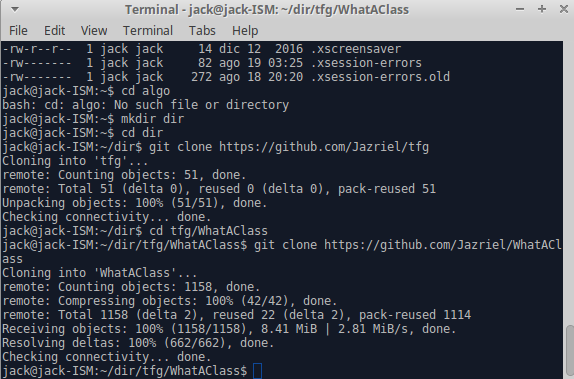
\includegraphics[width=1.0\textwidth]{shgit.png}
	\caption{Clonación de los repositorios}\label{fig:shgit.png}
\end{figure}


\subsection{Entorno virtual e instalación de las dependencias}

Una vez tenemos el código fuente es muy recomendable instalar las dependencias en un entorno virtual para evitar conflictos con otros proyectos.

\begin{lstlisting}[language=bash]
    $ cd WhatAClass
    $ virtualenv -p /usr/bin/python<VERSION> <DIR>
    $ source <DIR>/bin/activate
    $ pip install -r requirements.txt
\end{lstlisting}
\begin{figure}
	\centering
	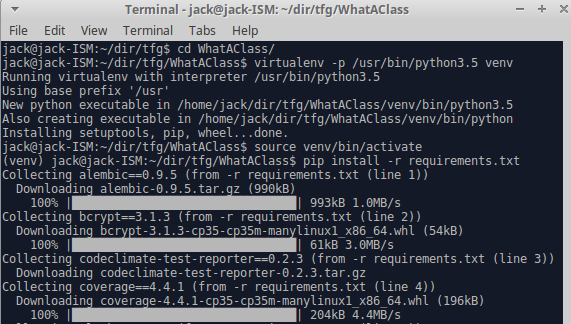
\includegraphics[width=1.0\textwidth]{shvenv.png}
	\caption{Creación de entorno virtual e instalación de dependencias}\label{fig:shvenv.png}
\end{figure}

Otra forma de instalar las dependencias es usando el archivo `setup.py', este archivo está pensado para poder usar pip como sistema de distribución del proyecto. No se ha visto necesario el subir el archivo a pip ya que no proporciona un servicio directo, sino que ayuda a proporcionar servicios. 

Para comprobar como funciona pip freeze para la actualización de dependencias, se expondrá a continuación un ejemplo ejecutado como continuación del anterior.

\begin{lstlisting}[language=bash]
    $ mkdir freeze
    $ cd freeze
    $ pip freeze > requirements.txt
\end{lstlisting}

\begin{figure}
	\centering
	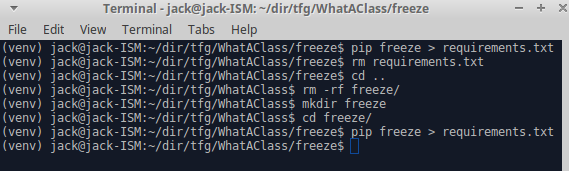
\includegraphics[width=1.0\textwidth]{shfreeze.png}
	\caption{Prueba de uso de pip freeze}\label{fig:shfreeze.png}
\end{figure}


Para actualizar las dependencias, como ya se ha comentado, solo debemos ejecutar este último comando y luego transcribirlo a `requirements.txt', normalmente con la \eng{pipe} igual que en el ejemplo anterior.

\subsection{Docker}

\lstset{style=linestyle}
\begin{lstlisting}[language=bash]
    $ docker build .
\end{lstlisting}

Para lanzar un contenedor y ponerlo en ejecución se puede hacer con el siguiente comando:

\lstset{style=linestyle}
\begin{lstlisting}[language=bash]
    $ docker run -i -t <image_id>
\end{lstlisting}

O el siguiente, si queremos usar el nombre del contenedor:

\lstset{style=linestyle}
\begin{lstlisting}[language=bash]
    $ docker run -i -t <image_name>:<version>
\end{lstlisting}

Si no nos acordásemos de que imágenes o que nombres tienen, ya que es difícil de acordarnos tanto de las ids como de los nombres auto-generados, podemos usar:

\lstset{style=linestyle}
\begin{lstlisting}[language=bash]
    $ docker images
\end{lstlisting}

Para todos estos comandos existen muchas variaciones, pero para su uso básico esta información es suficiente.

\subsubsection{Docker compose}

Para coordinar varios contenedores en el momento que queramos ejecutar la aplicación debemos usar un servicio de orquestración, como ya estamos usando docker, la opción más fácil y, de momento, profesional es docker compose.

La forma de usar docker compose es con un archivo `docker-compose.yml'. En el se especifican todas las configuraciones adicionales que se necesiten. 

Una vez tenemos nuestro archivo `docker-compose.yml' podemos usar los siguientes comandos para hacer la construcción de los contenedores y para desplegarlos:

\lstset{style=linestyle}
\begin{lstlisting}[language=bash]
    $ docker-compose build
    $ docker-compose up
\end{lstlisting}

\section{Instalación para uso local}
\label{sec:ins}
 
Esta instalación esta pensada para usuarios avanzados que quieran usar el servicio en local.

\begin{enumerate}
\setlength{\itemsep}{1pt}
\setlength{\parskip}{0pt}
\setlength{\parsep}{0pt}
\item Se debe comprobar que el ordenador permita la virtualización.
\item Instalar un navegador.
\item Instalar \hfoot{https://docs.docker.com/engine/installation/}{Docker CE}
\item Descargar este archivo \hfoot{https://raw.githubusercontent.com/Jazriel/TFG/master/docker-compose-hub/docker-compose.yml}{Docker compose}.
\item Ejecutar el siguiente comando en un lugar con acceso a internet.

\lstset{style=linestyle}
\begin{lstlisting}[language=bash]
    $ docker-compose pull 
\end{lstlisting}

\item Levantar el servicio con el comando posterior cuando queramos ejecutarlo.

\lstset{style=linestyle}
\begin{lstlisting}[language=bash]
    $ docker-compose up
\end{lstlisting}

\end{enumerate}

Si ejecutamos el 6 con internet se ejecutan tanto el 5 como el 6 ahorrando un mínimo de trabajo.

Cabe destacar que esta instalación es igual para windows y para linux.

Tras este proceso basta con acceder a 127.0.0.1 en el navegador.